% --------------------------------------------------------------------------- %
\subsection{Функциональные структуры данных}
% --------------------------------------------------------------------------- %
\begin{frame}
    \smaller[1]
    \begin{itemize}
        \item Были разработаны классы, представляющие функции-предикаты (Predicate), обработчики (Processor), селекторы (Selector) и функции перехода (Transfer).
        \item Для хранения данных был использован универсальный ассоциативный массив Anymap.
    \end{itemize}

    \begin{figure}
        \smaller[1]
        \centering
        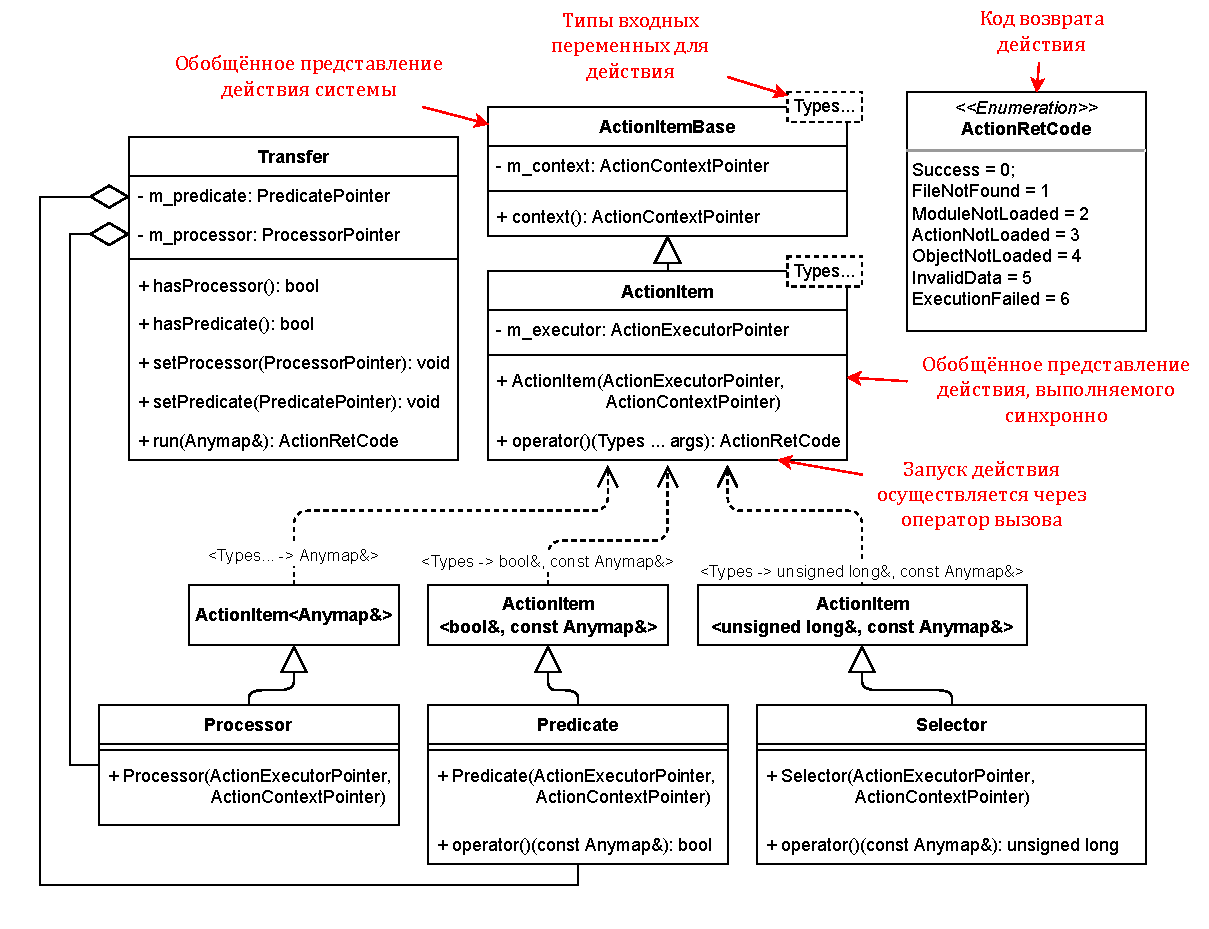
\includegraphics[height=0.64\textheight]{images/UML.graph_functions.pdf}
        \caption{UML-диаграмма разработанных функциональных структур данных}
    \end{figure}

\end{frame}
% --------------------------------------------------------------------------- %
\subsection{Информационные структуры данных}
% --------------------------------------------------------------------------- %
\begin{frame}

    \begin{itemize}
        \item Вершины графовой модели реализованы в классе Node.
        \item Рёбра графовой модели реализованы в классе Edge.
    \end{itemize}

    \begin{figure}
        \centering
        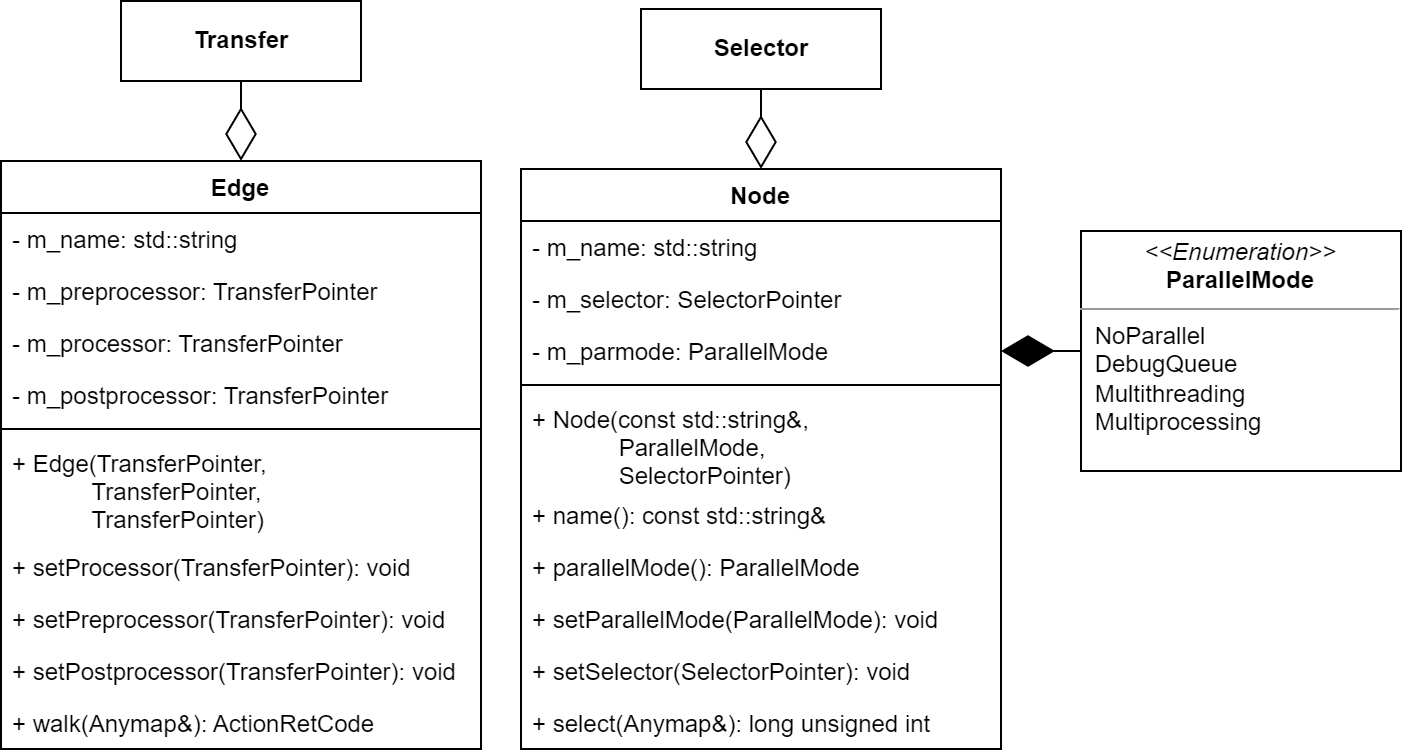
\includegraphics[height=0.6\textheight]{images/UML.graphElements.png}
        \caption{Разработанные структуры данных, представляющие элементы графовой модели}
    \end{figure}
\end{frame}

\begin{frame}

    \smaller[1]

    \begin{itemize}
        \item За программное представление графовых моделей отвечает класс Graph.
        \item Для объединения возможностей взаимодействия с вершинами и рёбрами и обращения к топологии графа спроектированы вспомогательные структуры данных NodeOp (операция с вершиной) и EdgeOp (операция с ребром).
    \end{itemize}

    \begin{figure}
        \begin{minipage}{0.38\textwidth}
            \centering
            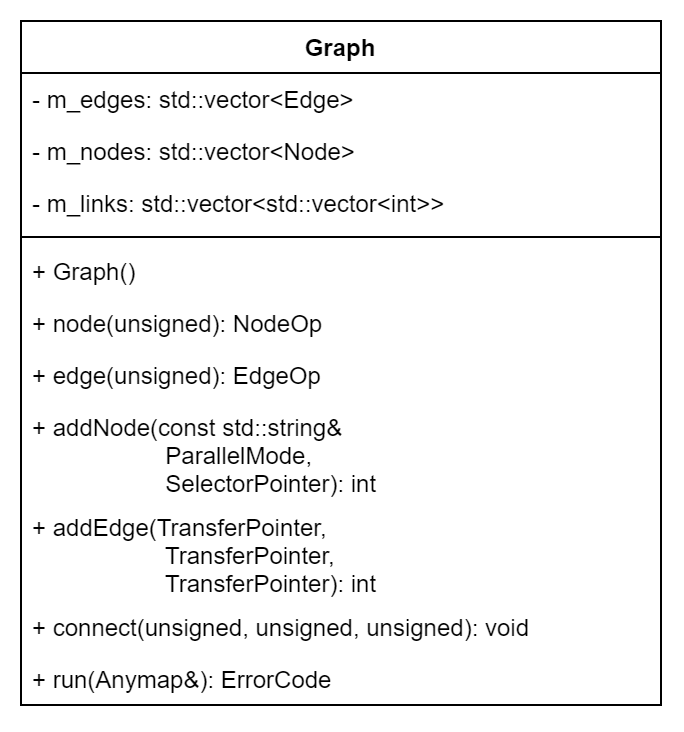
\includegraphics[width=\textwidth]{images/class.graph.png}
        \end{minipage}\hfill\begin{minipage}{0.62\textwidth}
            \centering
            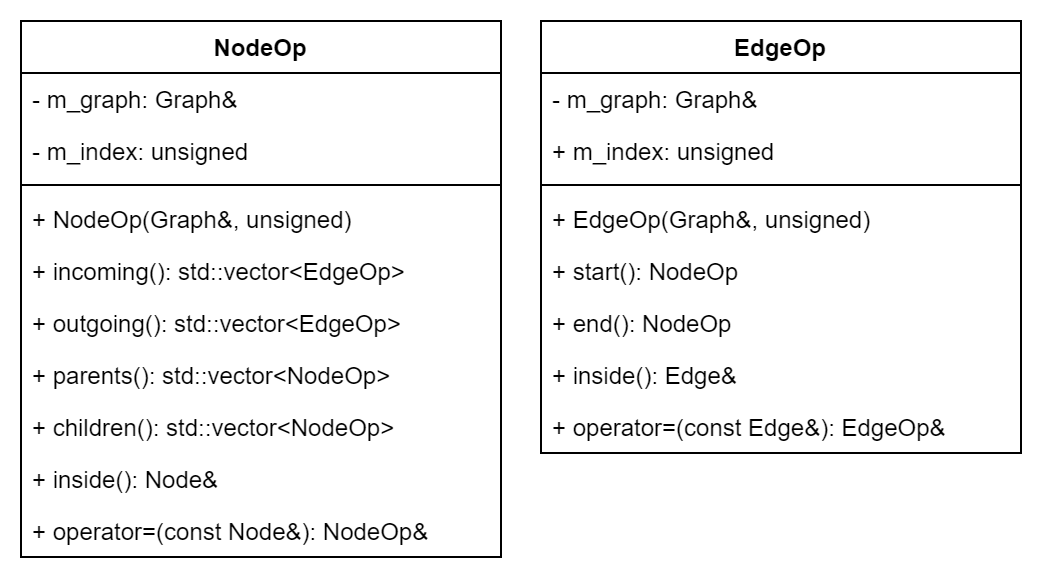
\includegraphics[width=\textwidth]{images/UML.topologyOperations.png}
        \end{minipage}
    \end{figure}


\end{frame}
% --------------------------------------------------------------------------- %
\subsection{Управляющие структуры данных}
% --------------------------------------------------------------------------- %
\begin{frame}
    \begin{itemize}
        \item Интерфейс ExecutionContainer отвечает за отслеживание выполнения параллельных ветвей графовой модели.
        \item Интерфейс ExecutionBranch отвечает за обход одной ветви графа и хранение вспомогательной информации о нём.
        \item ExecutionBranch уведомляет контейнер по завершении каждой функции перехода в обходимой ветви.
    \end{itemize}

    \begin{figure}
        \centering
        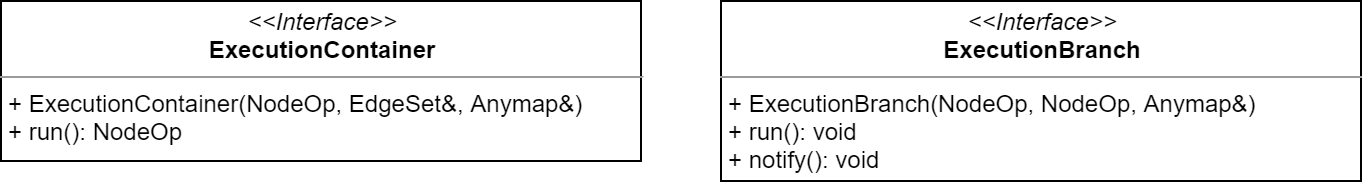
\includegraphics[width=0.75\textwidth]{images/UML.all.png}
        \caption{UML-диаграмма управляющих структур данных}
    \end{figure}


\end{frame}
% --------------------------------------------------------------------------- %
\subsection{Алгоритм обхода графовой модели}
\begin{frame}
    Приведённый алгоритм реализован в методе run() класса Graph.

    \begin{figure}
        \centering
        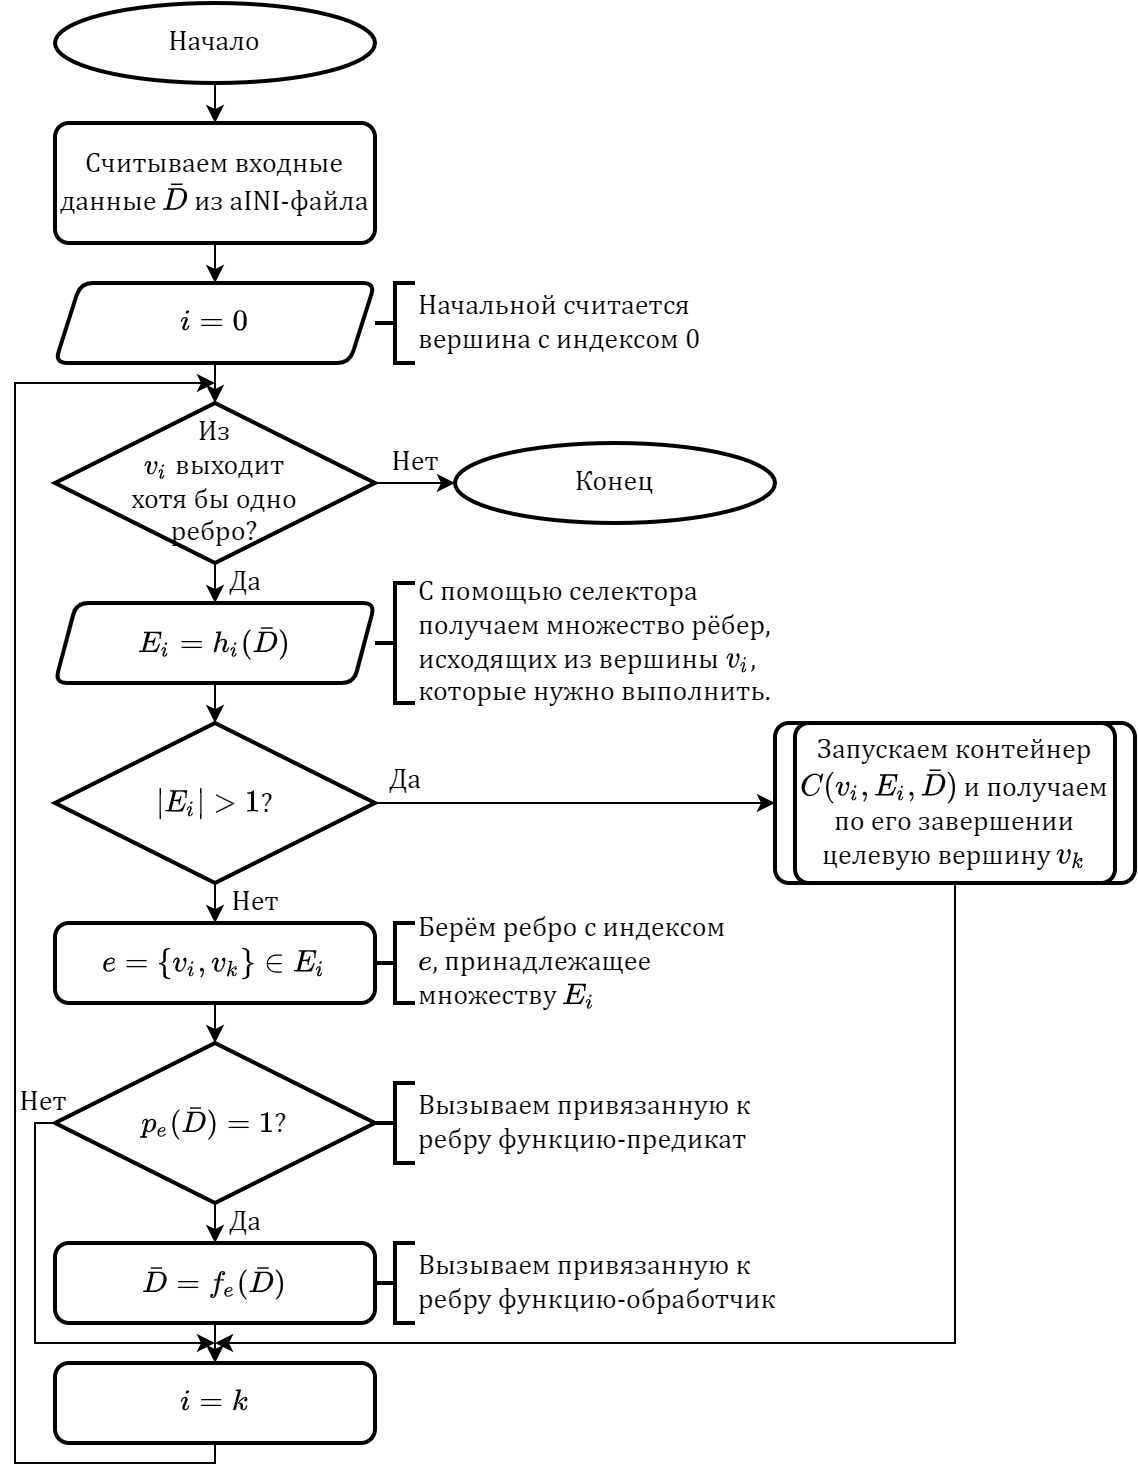
\includegraphics[height=0.7\textheight]{images/flowchart.graphRunning2.png}
        \caption{Общий алгоритм обхода графовой модели}
    \end{figure}
\end{frame}

\begin{frame}
    Приведённые ниже алгоритмы реализованы в методах run() классов ExecutionContainer и ExecutionBranch соответственно.

    \begin{figure}
        \begin{minipage}{0.35\textwidth}
            \centering
            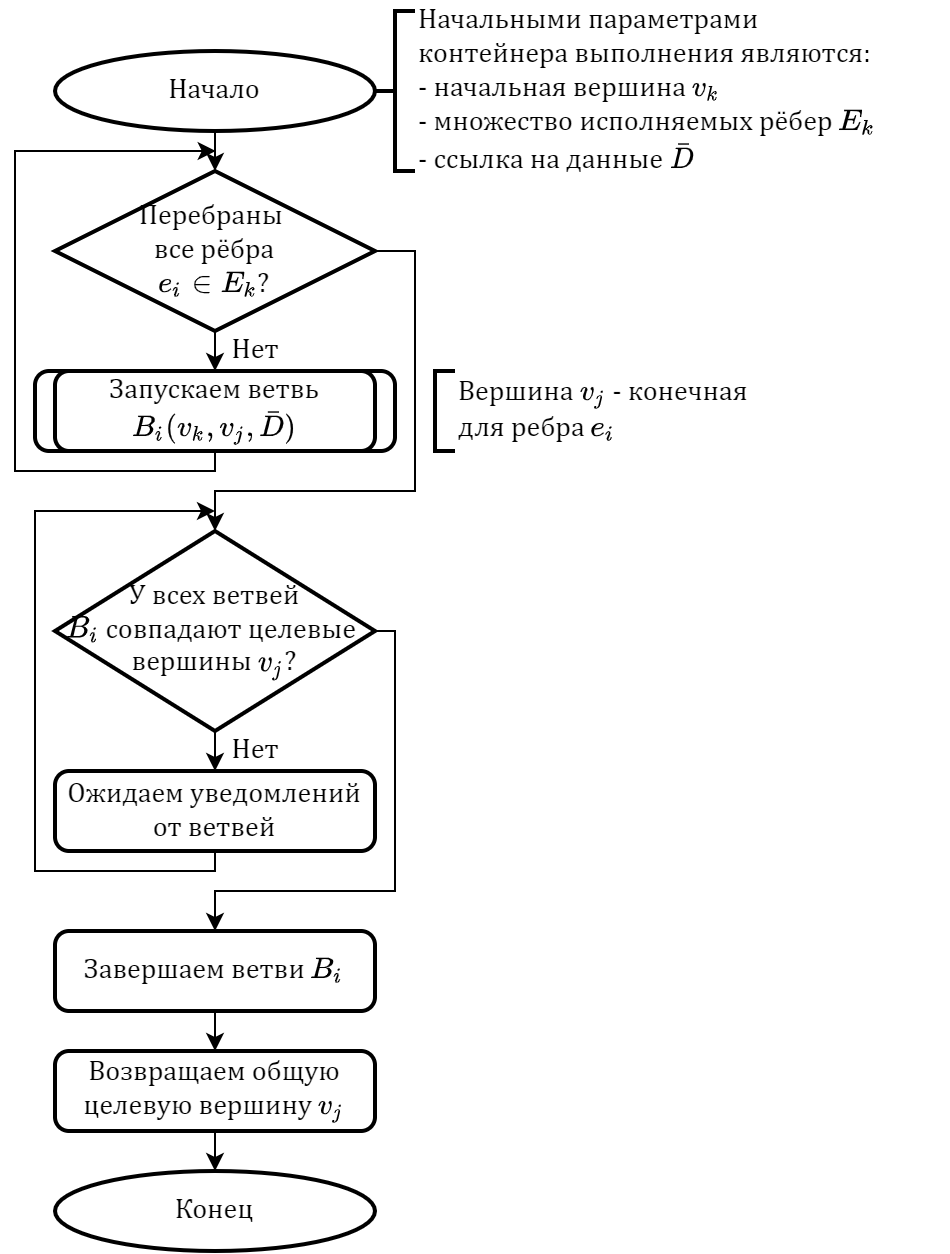
\includegraphics[height=0.6\textheight]{images/flowchart.executionContainer.png}
            \caption{Блок-схема алгоритма следящей структуры данных ``контейнер выполнения''}
        \end{minipage}\hfill\begin{minipage}{0.645\textwidth}
            \centering
            \includegraphics[width=\textwidth]{images/flowchart.executionBranch.png}
            \caption{Блок-схема алгоритма обхода одной ветви графовой модели}
        \end{minipage}
    \end{figure}

\end{frame}
